\documentclass[12pt]{article}
\usepackage[a4paper,width=150mm,top=20mm,bottom=20mm]{geometry}
\usepackage{amsmath}
\usepackage{graphicx}
\usepackage{hyperref}
\usepackage[utf8]{vietnam}

\title{\textbf{Báo cáo demo chương trình Homework 1 \linebreak Môn học: Lập Trình Mạng - IT4062}}

\author{Trương Minh Hồng - 20194576}

\date{\today}

\begin{document}

\maketitle

\section{Chạy chương trình}

\begin{itemize}

\item Giải nén file \textbf{TruongMinhHong{\_}20194576{\_}HW1.zip}.
\item Mở terminal tại folder vừa giải nén.
\item Chạy câu lệnh \textit{make}
\item Chạy câu lệnh \textit{./main}
\end{itemize}
Minh họa cách chạy chương trình.

\begin{figure}[h]
    \begin{center}
        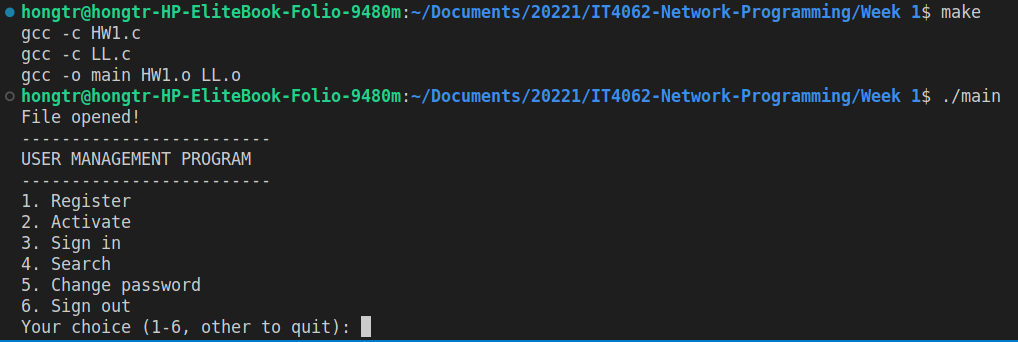
\includegraphics[width=0.8\linewidth]{Img/demo.png}
    \end{center}
    \caption{Chạy chương trình}
    \label{fig:demo}
  \end{figure}

Thông tin tài khoản có sẵn trong file \textit{nguoidung.txt}.

\begin{figure}[h]
    \begin{center}
        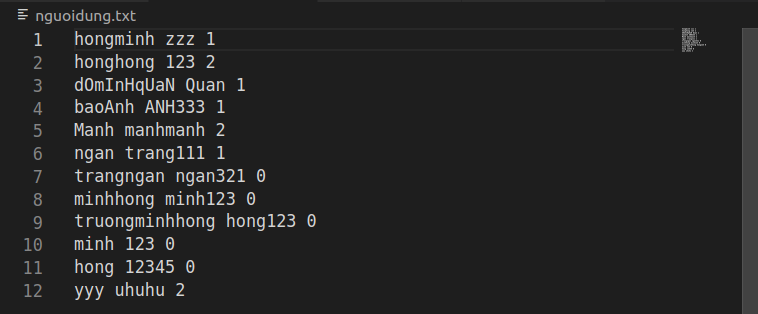
\includegraphics[width=0.8\linewidth, height=4.5cm]{Img/file.png}
    \end{center}
    \caption{Thông tin tài khoản}
    \label{fig:file}
\end{figure}
\section{Kiểm tra chức năng chương trình}
\subsection{Register}
Đăng kí tài khoản mới. Nếu username đã có trong file (ví du \textit{minhhong}) thì báo lỗi \textit{Account existed!}. Tài khoản mới có trạng thái hoạt động là \textbf{idle}.
\begin{figure}[h]
    \begin{center}
        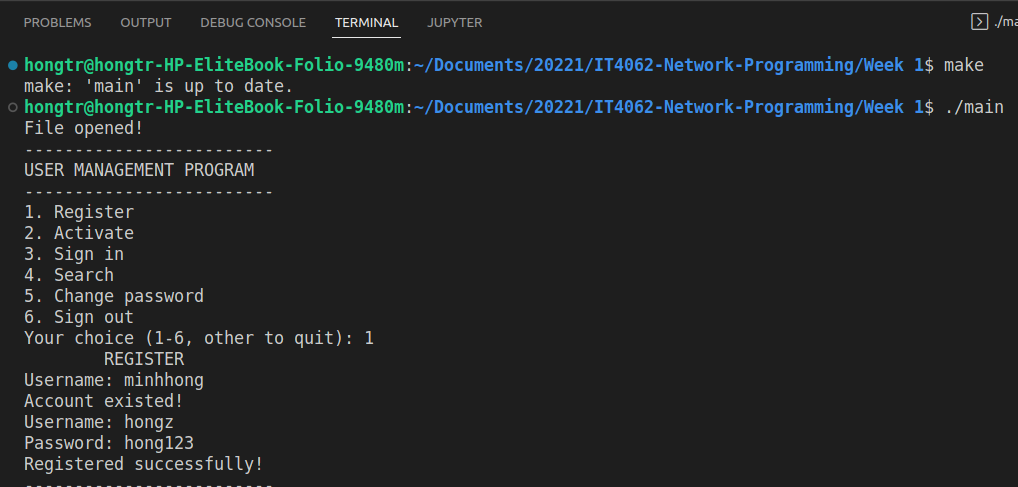
\includegraphics[width=0.8\linewidth, height=4.5cm]{Img/1_chay.png}
    \end{center}
    \caption{Đăng kí tài khoản}
    \label{fig:1_chay}
\end{figure}
\begin{figure}[h]
    \begin{center}
        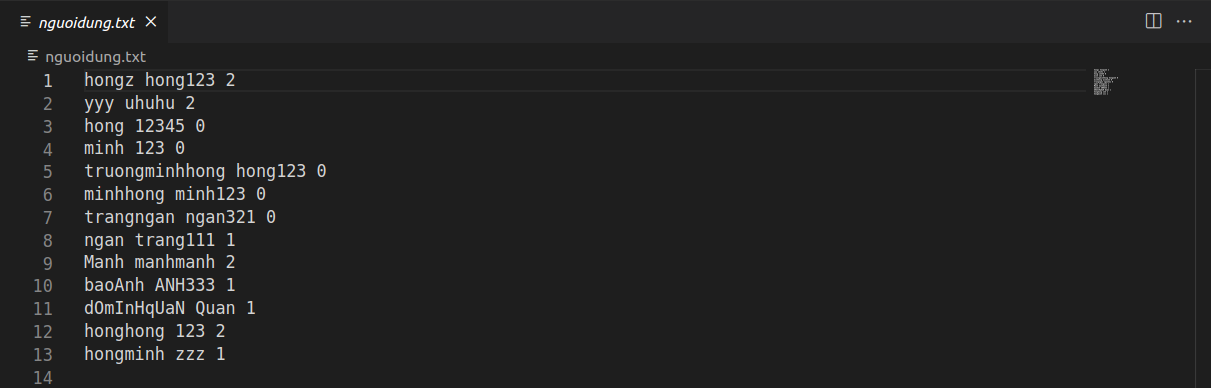
\includegraphics[width=0.8\linewidth, height=4.5cm]{Img/1_data.png}
    \end{center}
    \caption{Tài khoản mới được thêm vào file}
    \label{fig:1_file}
\end{figure}

\subsection{Activate}
Kích hoạt tài khoản. Sai mã kích hoạt báo lỗi, sai quá 4 lần tài khoản sẽ bị khóa. \linebreak Nếu đúng mã kích hoạt \textit{20194576} tài khoản chuyển sang trạng thái active.

\begin{figure}[h]
    \begin{center}
        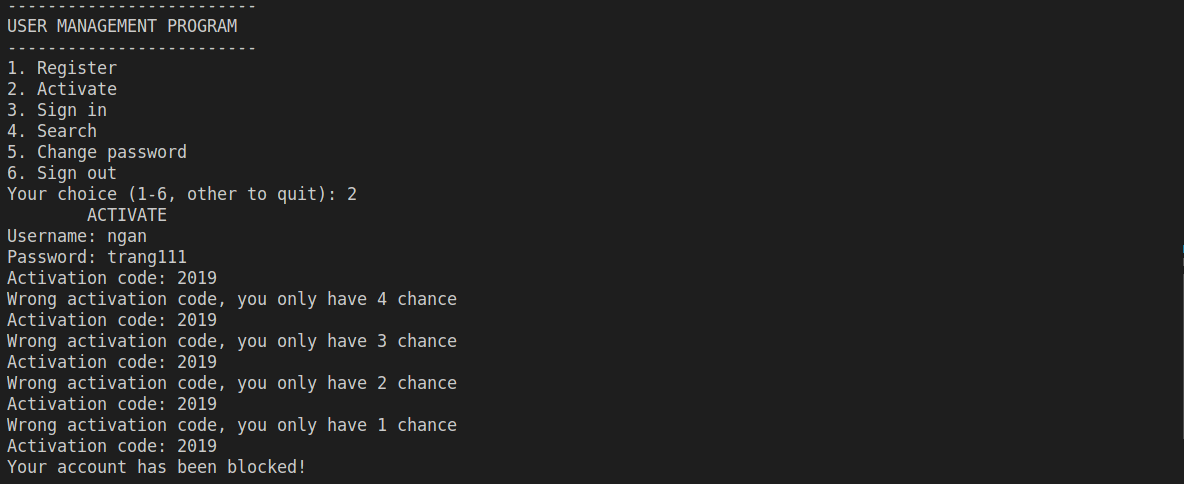
\includegraphics[width=0.8\linewidth, height=4.5cm]{Img/Thu4Lan.png}
    \end{center}
    \caption{Nhập sai quá 4 lần mã kích hoạt.}
    \label{fig:2_nhapsai}
\end{figure}
\begin{figure}[h]
    \begin{center}
        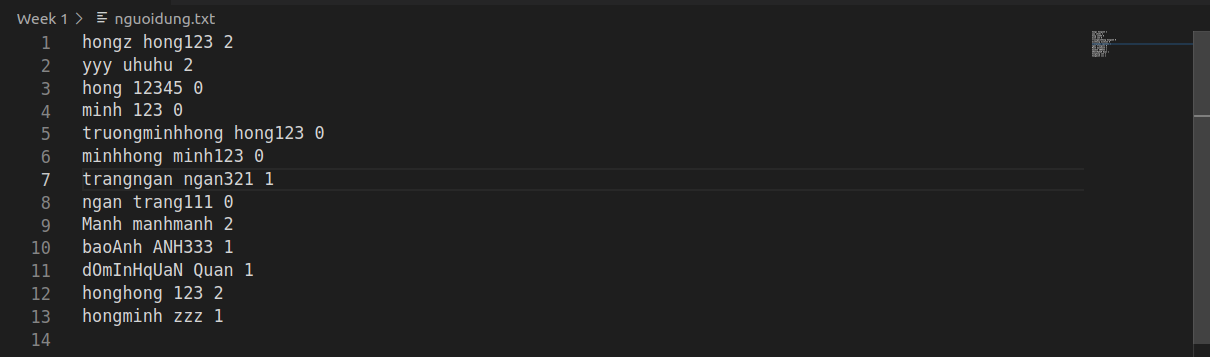
\includegraphics[width=0.8\linewidth, height=4.5cm]{Img/Truockhikhoa.png}
    \end{center}
    \caption{Tài khoản trước khi khóa (hàng 7)}
    \label{fig:2_truoc}
\end{figure}

\begin{figure}[h]
    \begin{center}
        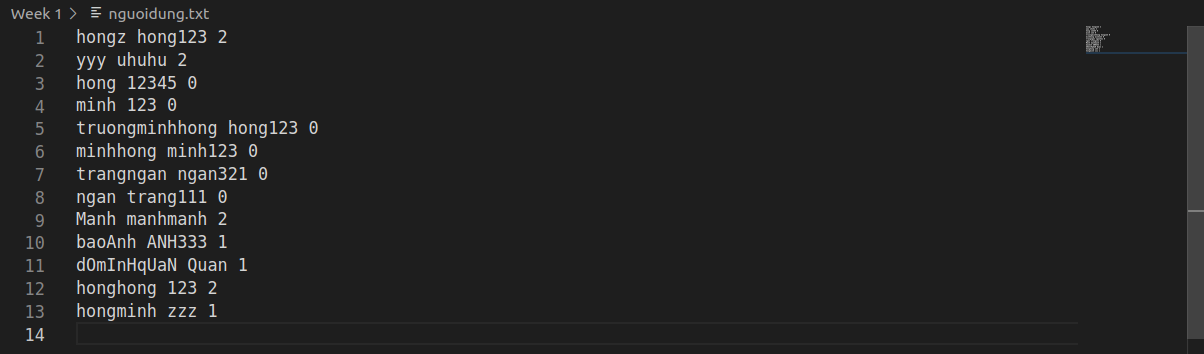
\includegraphics[width=0.8\linewidth, height=4.5cm]{Img/Saukhikhoa.png}
    \end{center}
    \caption{Tài khoản sau khi khóa (hàng 7)}
    \label{fig:2_sau}
\end{figure}

Nếu kích hoạt thành công, tài khoản chuyển sang chế độ active.
\begin{figure}[!htb]
    \begin{center}
        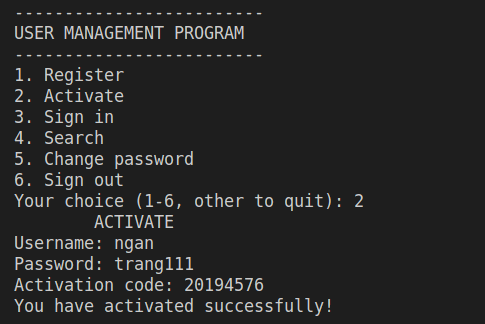
\includegraphics[width=0.8\linewidth, height=4.5cm]{Img/2_thanhcong.png}
    \end{center}
    \caption{Kích hoạt tài khoản thành công}
    \label{fig:2_thanhcong}
\end{figure}
\begin{figure}[!htb]
    \begin{center}
        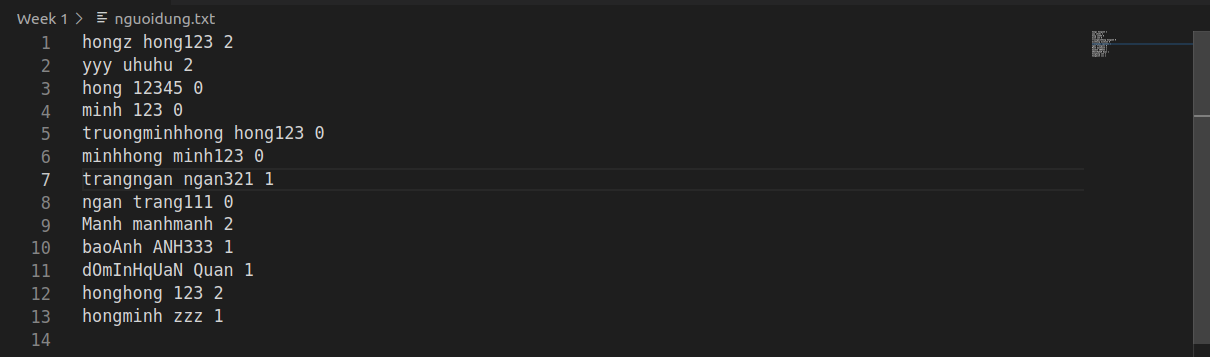
\includegraphics[width=0.8\linewidth, height=4.5cm]{Img/Truockhikhoa.png}
    \end{center}
    \caption{Tài khoản sau khi kích hoạt thành công (hàng 7)}
    \label{fig:2_filethanhcong}
\end{figure}

\subsection{Sign in}
\begin{figure}[h]
    \begin{center}
        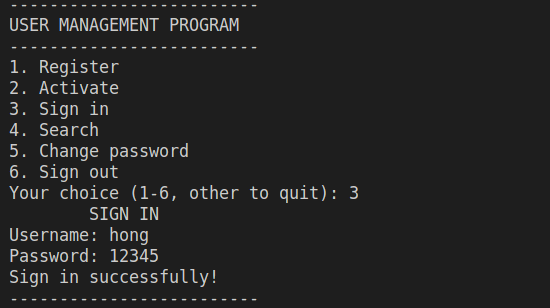
\includegraphics[width=0.8\linewidth, height=4.5cm]{Img/3_thanhcong.png}
    \end{center}
    \caption{Đăng nhập thành công}
    \label{fig:3_filethanhcong}
\end{figure}

\subsection{Search}
Tìm kiếm thông tin tài khoản. Nếu không có tài khoản thì báo lỗi.Nếu có tài khoản, in ra trạng thái tương ứng.
\begin{figure}[!htb]
    \begin{center}
        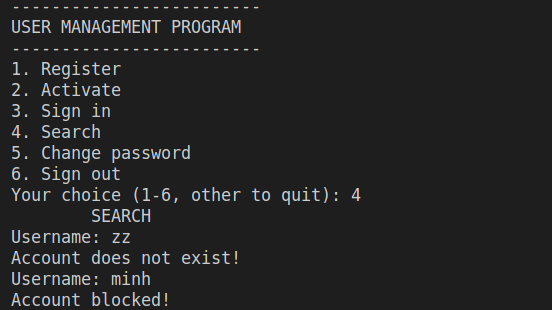
\includegraphics[width=0.8\linewidth, height=4.5cm]{Img/4.png}
    \end{center}
    \caption{Tìm kiếm tài khoản}
    \label{fig:4_filethanhcong}
\end{figure}

\subsection{Change password}
Chỉ thay đổi được password những tài khoản đã được kích hoạt (status = 1). Chương trình cũng có thể kiểm tra mật khẩu cũ trước khi đổi mật khẩu (chỉ được sai dưới 3 lần).
\begin{figure}[!htb]
    \begin{center}
        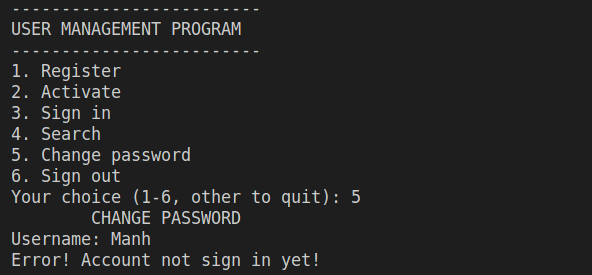
\includegraphics[width=0.8\linewidth, height=4.5cm]{Img/5fail.png}
    \end{center}
    \caption{Không thay đổi được mật khẩu tài khoản chưa kích hoạt}
    \label{fig:5_khoa}
\end{figure}
\begin{figure}[!htb]
    \begin{center}
        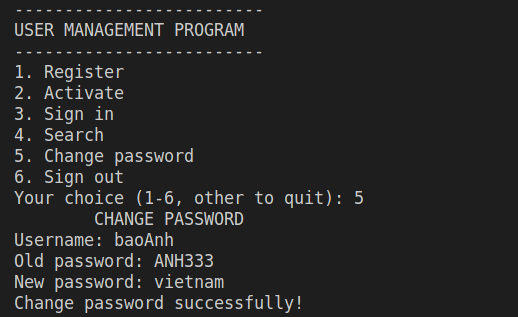
\includegraphics[width=0.8\linewidth, height=4.5cm]{Img/5suc.png}
    \end{center}
    \caption{Thay đổi mật khẩu thành công}
    \label{fig:5_suc}
\end{figure}
\begin{figure}[!htb]
    \begin{center}
        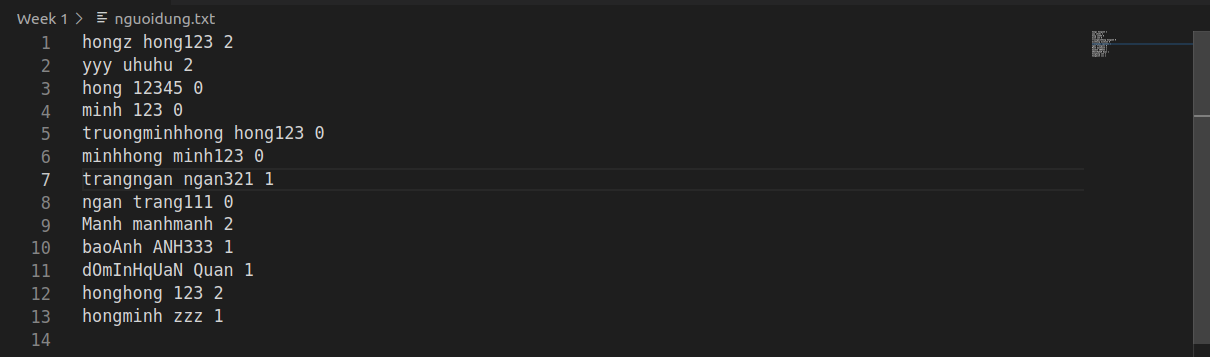
\includegraphics[width=0.8\linewidth, height=4.5cm]{Img/Truockhikhoa.png}
    \end{center}
    \caption{Tài khoản trước khi thay đổi mật khẩu (hàng 10)}
    \label{fig:5_akhoa}
\end{figure}
\begin{figure}[!htb]
    \begin{center}
        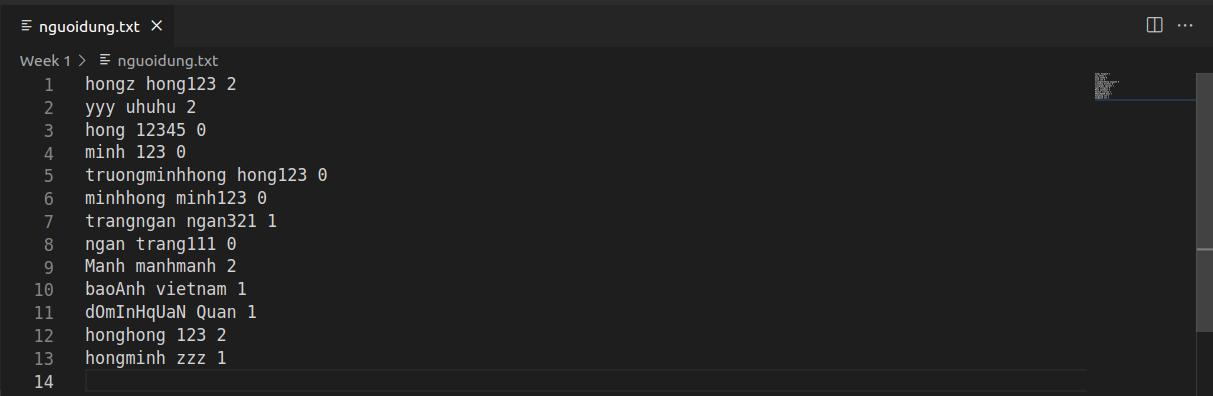
\includegraphics[width=0.8\linewidth, height=4.5cm]{Img/5sucfile.png}
    \end{center}
    \caption{Tài khoản sau khi thay đổi mật khẩu (hàng 10)}
    \label{fig:5_sucfile}
\end{figure}

\newpage
\subsection{Sign out}
\begin{figure}[!htb]
    \begin{center}
        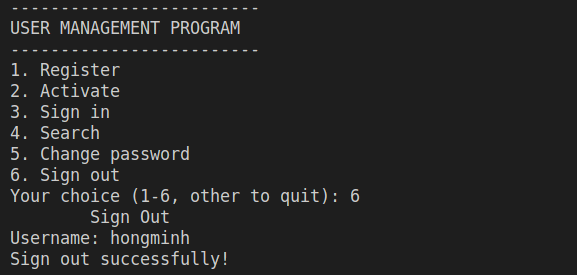
\includegraphics[width=0.8\linewidth, height=4.5cm]{Img/6Sign.png}
    \end{center}
    \caption{Đăng xuất thành công}
    \label{fig:6_sucfile}
\end{figure}

\end{document}
